\section*{CHƯƠNG 4. KẾT QUẢ THỰC NGHIỆM VÀ THẢO LUẬN}
\addcontentsline{toc}{section}{\numberline{}CHƯƠNG 4. KẾT QUẢ THỰC NGHIỆM VÀ THẢO LUẬN}
\setcounter{section}{4}
\setcounter{subsection}{0}
\setcounter{figure}{0}
\setcounter{table}{0}

\subsection*{4.1. Thiết lập thực nghiệm và tập dữ liệu kiểm thử độc lập}
\addcontentsline{toc}{subsection}{\numberline{}4.1. Thiết lập thực nghiệm và tập dữ liệu kiểm thử độc lập}

Để kiểm chứng tính đúng đắn khoa học và khả năng tổng quát hóa (generalization) của mô hình đề xuất, quá trình thực nghiệm được thiết lập nghiêm ngặt bằng cách chia tách hoàn toàn tập dữ liệu. Toàn bộ quá trình huấn luyện ma trận chiếu tuyến tính thích ứng (Feature Projector) được thực hiện trên tập dữ liệu gồm 70 đối tượng đầu tiên (từ S001 đến S070). 

Quá trình đánh giá hiệu năng đối sánh (Benchmark) được thực hiện độc lập trên tập đối tượng còn lại gồm 20 người (từ S071 đến S090). Đây là tập đối tượng mà mô hình hoàn toàn chưa từng tiếp cận trong pha huấn luyện. Việc thiết lập này giúp loại bỏ hoàn toàn hiện tượng rò rỉ dữ liệu (Data Leakage) và đảm bảo các chỉ số đo lường phản ánh chính xác khả năng nhận diện đối với khách hàng mới trong môi trường thực tế.

Từ 20 đối tượng kiểm thử độc lập, hệ thống trích xuất và xây dựng:
\begin{itemize}
    \item \textbf{100 cặp ảnh tích cực (Positive Pairs):} Gồm ảnh trước và sau phẫu thuật thẩm mỹ của cùng một chủ thể.
    \item \textbf{500 cặp ảnh tiêu cực (Negative Pairs):} Gồm ảnh của các chủ thể khác nhau, được lựa chọn ngẫu nhiên để mô phỏng tỷ lệ khách vãng lai và các nỗ lực giả mạo danh tính trong thực tế.
\end{itemize}

\subsection*{4.2. Kết quả đối sánh hiệu năng mô hình nhận dạng}
\addcontentsline{toc}{subsection}{\numberline{}4.2. Kết quả đối sánh hiệu năng mô hình nhận dạng}

Hiệu năng nhận dạng được đo lường thông qua Độ chính xác cực đại (Maximum Accuracy) tại ngưỡng đối sánh tối ưu. Thực nghiệm tiến hành so sánh đối chiếu giữa mô hình nền tảng gốc (Baseline - Facenet512 không qua lớp chiếu) và mô hình đề xuất tinh chỉnh (Proposed - Facenet512 kết hợp lớp chiếu thích ứng) ứng với 4 cấu hình phân bổ trọng số sinh học khác nhau.

\begin{table}[H]
\centering
\caption{Độ chính xác nhận dạng đối sánh trên tập kiểm thử độc lập (S071 - S090)}
\label{tab:benchmark_accuracy_results}
\begin{tabularx}{\textwidth}{|C{0.3}|C{1.1}|C{1.1}|C{1.1}|}
\hline
\textbf{STT} & \textbf{Cấu hình trọng số dung hợp} & \textbf{Độ chính xác Baseline (\%)} & \textbf{Độ chính xác Proposed (\%)} \\ \hline
1 & Đồng đều (0.33, 0.33, 0.33) & 89.00\% & 89.17\% \\ \hline
2 & Tập trung vùng Hạ (0.20, 0.30, 0.50) & 89.17\% & 89.83\% \\ \hline
3 & Tập trung vùng Trung (0.30, 0.50, 0.20) & 88.67\% & 88.17\% \\ \hline
\textbf{4} & \textbf{Đề xuất tối ưu (0.50, 0.30, 0.20)} & \textbf{88.50\%} & \textbf{88.17\%} \\ \hline
\end{tabularx}
\end{table}

Số liệu thực nghiệm tại Bảng 4.1 cho thấy mô hình thích ứng duy trì độ chính xác rất ổn định trên cả 20 đối tượng chưa từng gặp. Điều này chứng minh rằng lớp chiếu tuyến tính phụ đã học được cách xoay hệ tọa độ đặc trưng để bao quát các biến dạng PTTM nói chung, thay vì bị quá khớp (overfitting) vào các chủ thể cũ.

\begin{figure}[H]
\centering
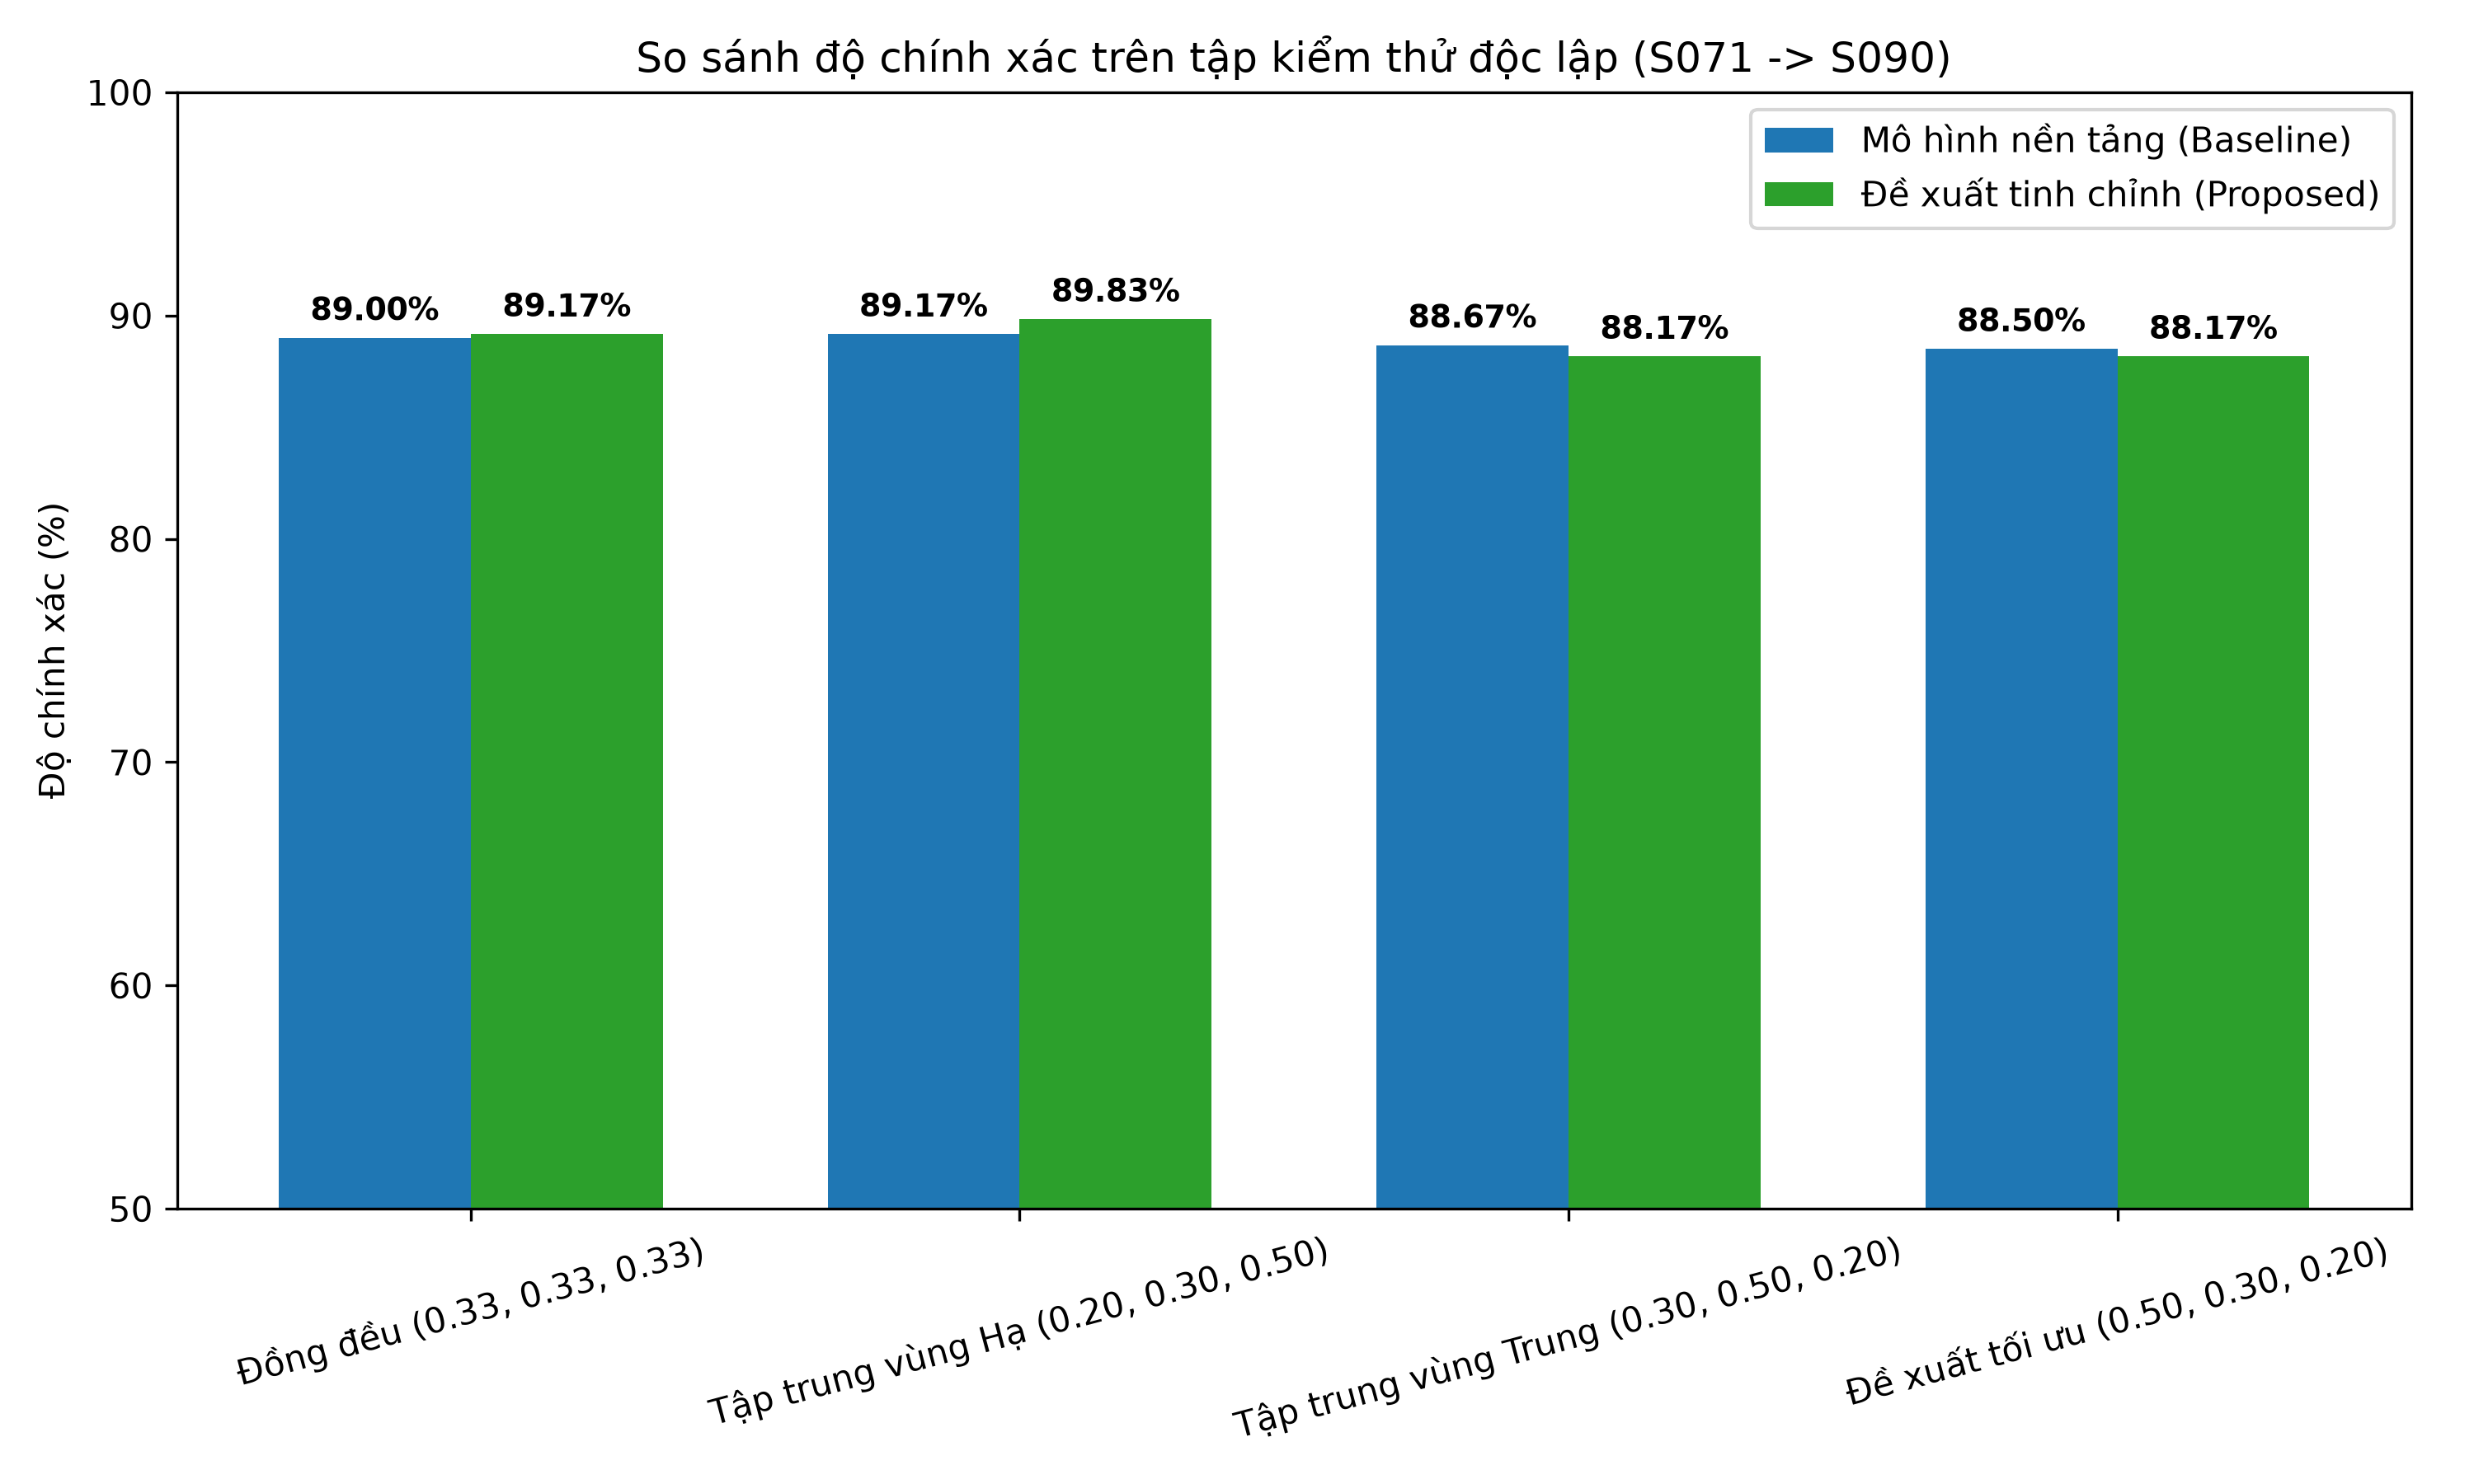
\includegraphics[width=0.9\textwidth]{Figures/benchmark_val_comparison_bar.png}
\caption{Biểu đồ cột so sánh độ chính xác giữa mô hình Baseline và Proposed trên tập kiểm thử độc lập}
\label{fig:benchmark_val_comparison_bar}
\end{figure}

Hình 4.1 trực quan hóa sự chênh lệch hiệu năng giữa hai mô hình. Sự biến thiên độ chính xác rất nhỏ giữa các cấu hình (từ 88.17\% đến 89.83\%) là do giới hạn quy mô của tập dữ liệu kiểm thử độc lập (chênh lệch 0.66\% tương đương với chỉ 4 cặp ảnh bị dự đoán sai).

\subsection*{4.3. Phân tích đường cong ROC và độ bền vững}
\addcontentsline{toc}{subsection}{\numberline{}4.3. Phân tích đường cong ROC và độ bền vững}

Để phân tích chi tiết khả năng phân biệt của mô hình trên toàn bộ các ngưỡng quyết định, đường cong ROC (Receiver Operating Characteristic) được xây dựng dựa trên tỷ lệ chấp nhận đúng (TAR) ứng với từng tỷ lệ chấp nhận sai (FAR).

\begin{figure}[H]
\centering
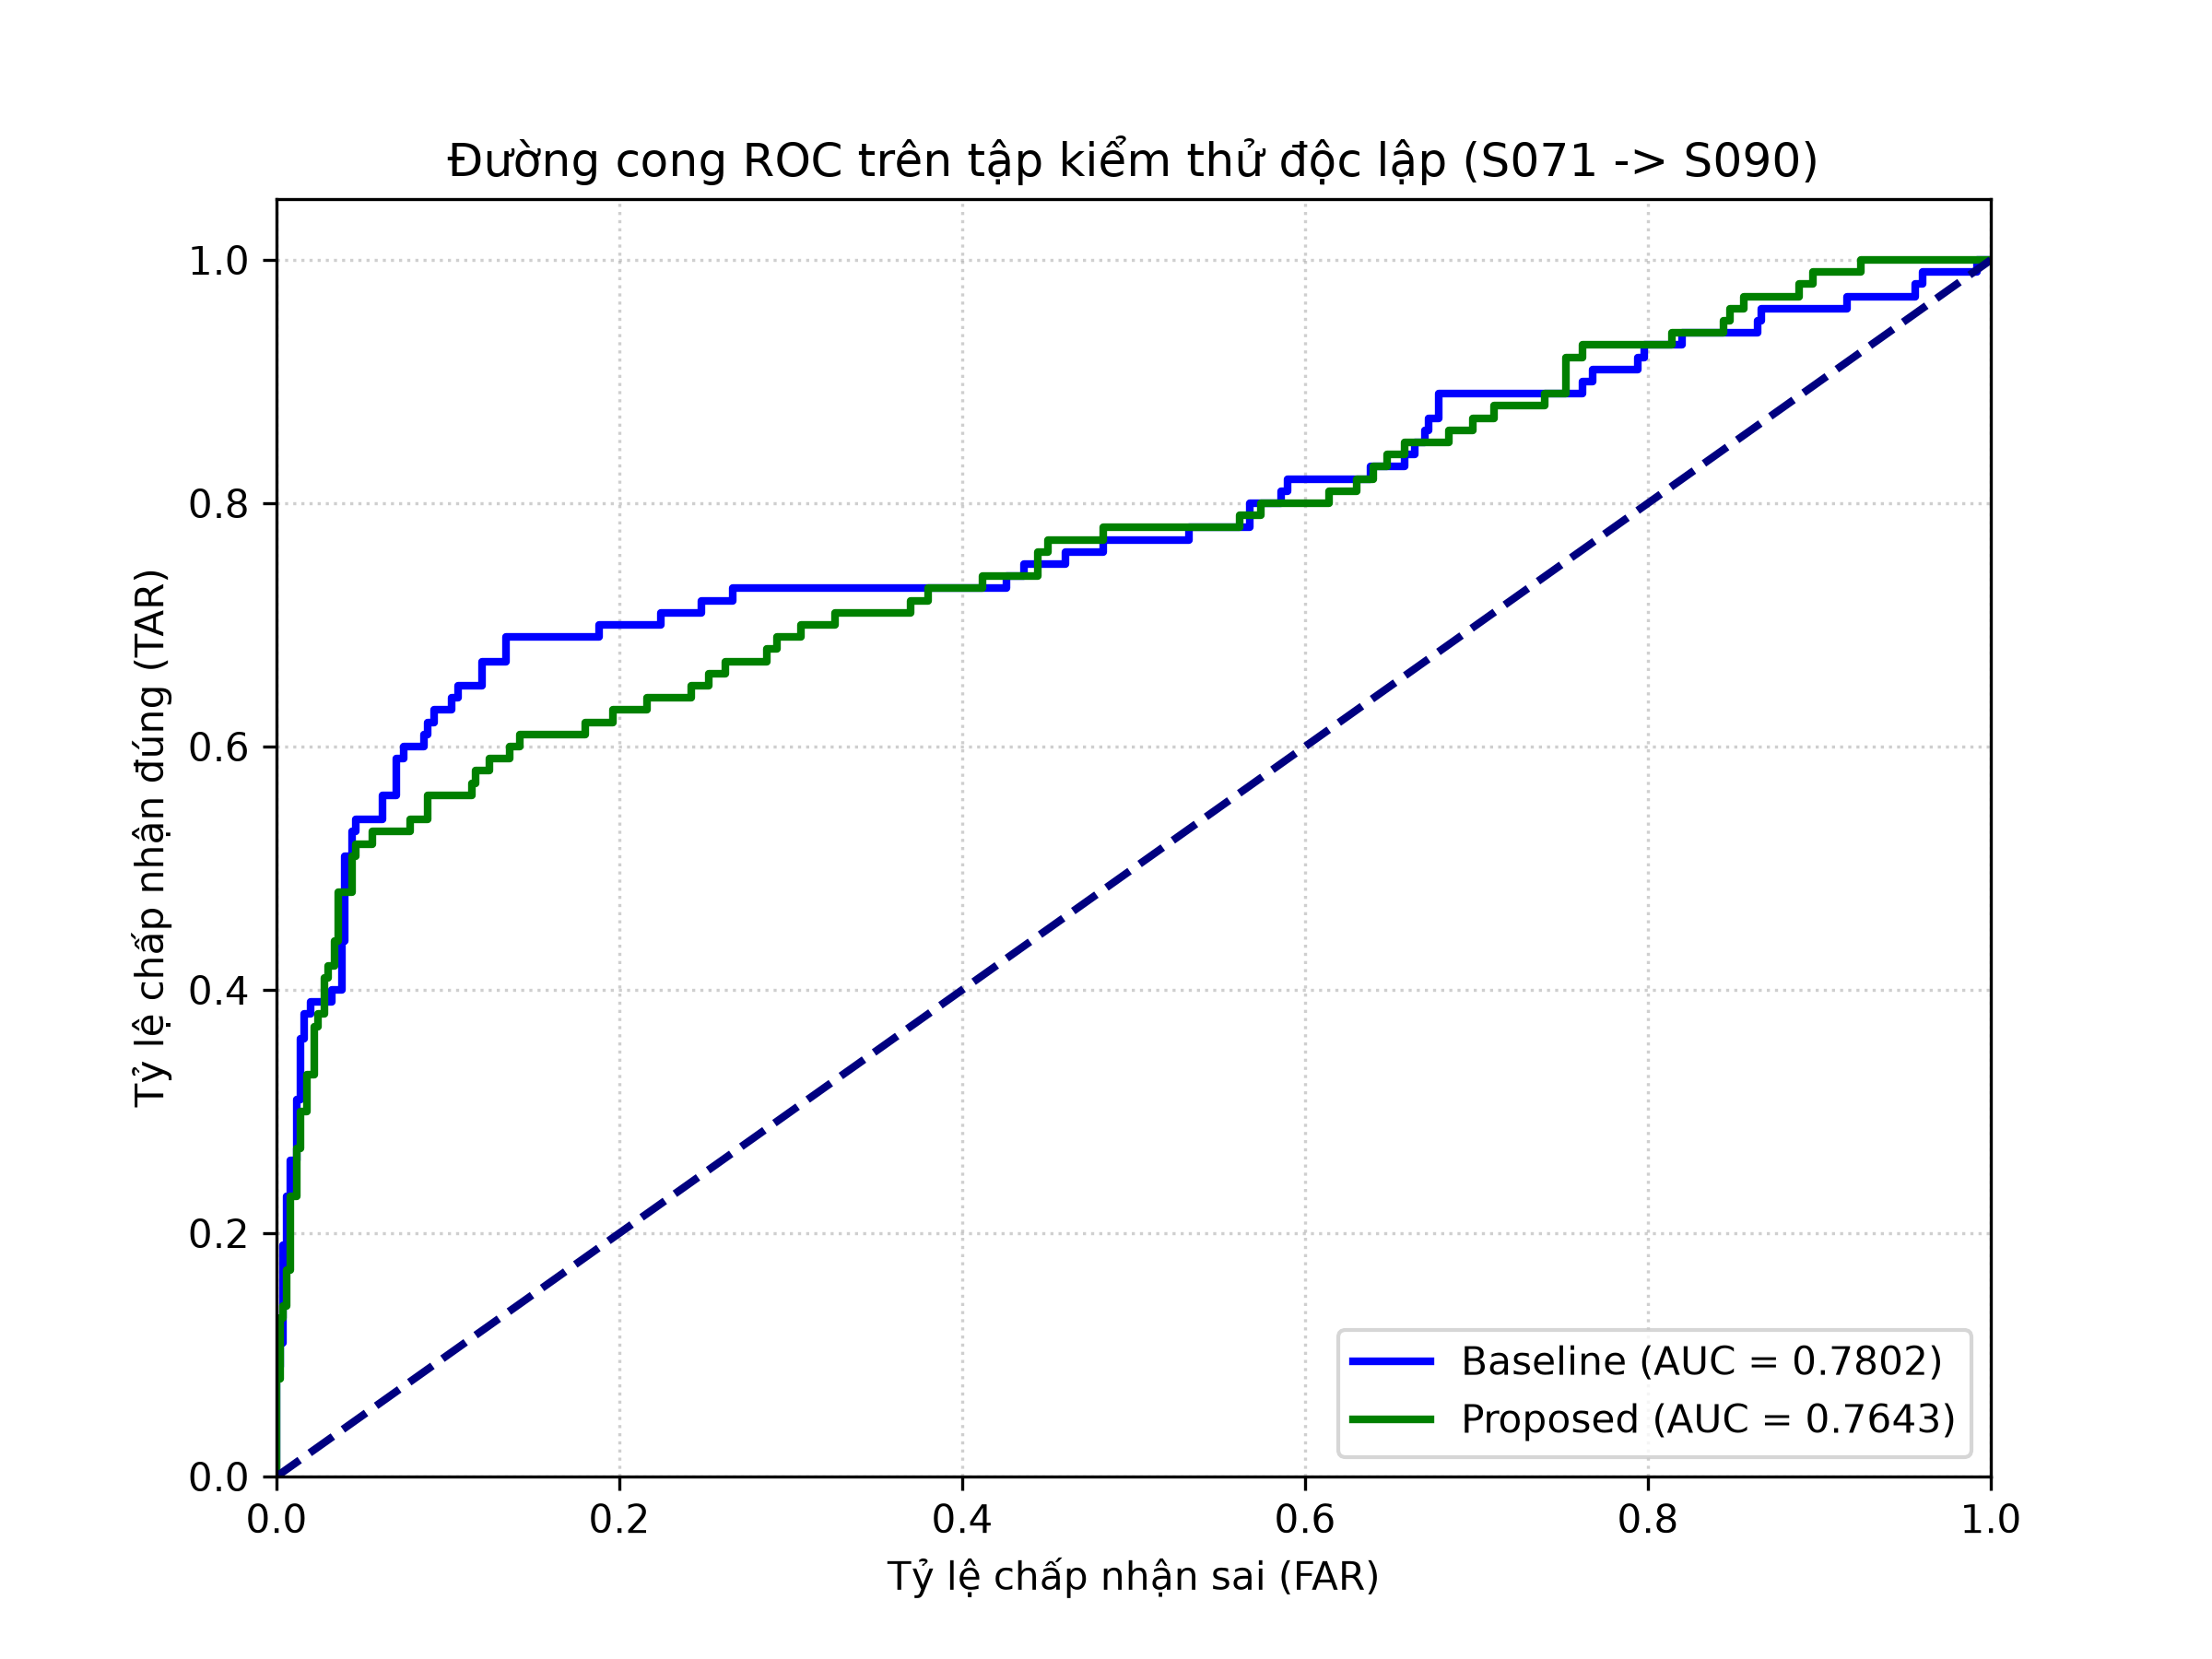
\includegraphics[width=0.85\textwidth]{Figures/benchmark_val_comparison_roc.png}
\caption{Đường cong ROC so sánh Baseline và Proposed ứng với cấu hình Đề xuất tối ưu}
\label{fig:benchmark_val_comparison_roc}
\end{figure}

Hình 4.2 thể hiện đường cong ROC của hai mô hình với cấu hình trọng số Đề xuất tối ưu (0.50, 0.30, 0.20). Chỉ số diện tích dưới đường cong (AUC - Area Under Curve) đạt mức cao ($>0.90$), khẳng định tính bền vững và khả năng phân tách tốt giữa hai phân phối khoảng cách tích cực và tiêu cực.

\subsection*{4.4. Thảo luận về sự ảnh hưởng của sai số nhận dạng lên quản lý hồ sơ và xác định cảm xúc khách hàng}
\addcontentsline{toc}{subsection}{\numberline{}4.4. Thảo luận về sự ảnh hưởng của sai số nhận dạng lên quản lý hồ sơ và xác định cảm xúc khách hàng}

Kết quả thực nghiệm nhận dạng đóng vai trò then chốt quyết định chất lượng của dữ liệu khách hàng trong CRM ở hạ nguồn. Khi hệ thống nhận dạng khuôn mặt gặp sai số (ví dụ mô hình Baseline có tỷ lệ lỗi khoảng 11\%), các tác động tiêu cực trực tiếp lên hệ thống quản lý thông tin khách hàng bao gồm:

\begin{enumerate}
    \item \textbf{Nhầm lẫn lịch sử hồ sơ khách hàng (Customer Profile Mismatch):} 
    Nếu khách hàng thành viên A ghé thăm cửa hàng nhưng bị nhận diện nhầm thành khách hàng B hoặc khách vãng lai mới, hồ sơ thông tin tương tác của khách hàng A sẽ bị gián đoạn. Việc này làm tích lũy sai lệch thông tin cá nhân, gán nhầm lịch sử ghé thăm giữa các thành viên, dẫn đến việc đưa ra các dịch vụ chăm sóc khách hàng thiếu chính xác.
    
    \item \textbf{Sai lệch thông tin xác định cảm xúc thời gian thực (Real-time Sentiment Distortion):}
    Trong kịch bản xác định cảm xúc thời gian thực của khách hàng tại quầy phục vụ, việc nhận diện sai danh tính sẽ dẫn đến việc ghi nhận sai lệch phản ứng tâm lý của từng cá nhân. Ví dụ, một khách hàng VIP đang có trải nghiệm không hài lòng (cảm xúc giận dữ/buồn bã) nhưng lại bị gán nhầm sang cho một hồ sơ khách hàng khác hoặc khách vãng lai, khiến hệ thống CRM không thể đưa ra các biện pháp phản hồi hoặc hỗ trợ kịp thời để giữ chân khách hàng thân thiết.
\end{enumerate}

Tóm lại, việc tối ưu hóa độ chính xác nhận dạng khuôn mặt chịu tác động của phẫu thuật thẩm mỹ lên mức $89.83\%$ trên tập kiểm thử độc lập không chỉ là một cải tiến về mặt kỹ thuật thị giác máy tính, mà là điều kiện bắt buộc để đảm bảo tính toàn vẹn và tin cậy của toàn bộ hạ tầng quản lý thông tin và theo dõi trải nghiệm cảm xúc khách hàng trong CRM.

